\documentclass[tikz,border=5pt,png]{standalone}
\usepackage{tikz}
\usetikzlibrary{shapes,backgrounds,calc}
\usepackage[utf8]{inputenc}
\usepackage[T1]{fontenc}
\renewcommand{\familydefault}{\sfdefault}

\begin{document}
	
	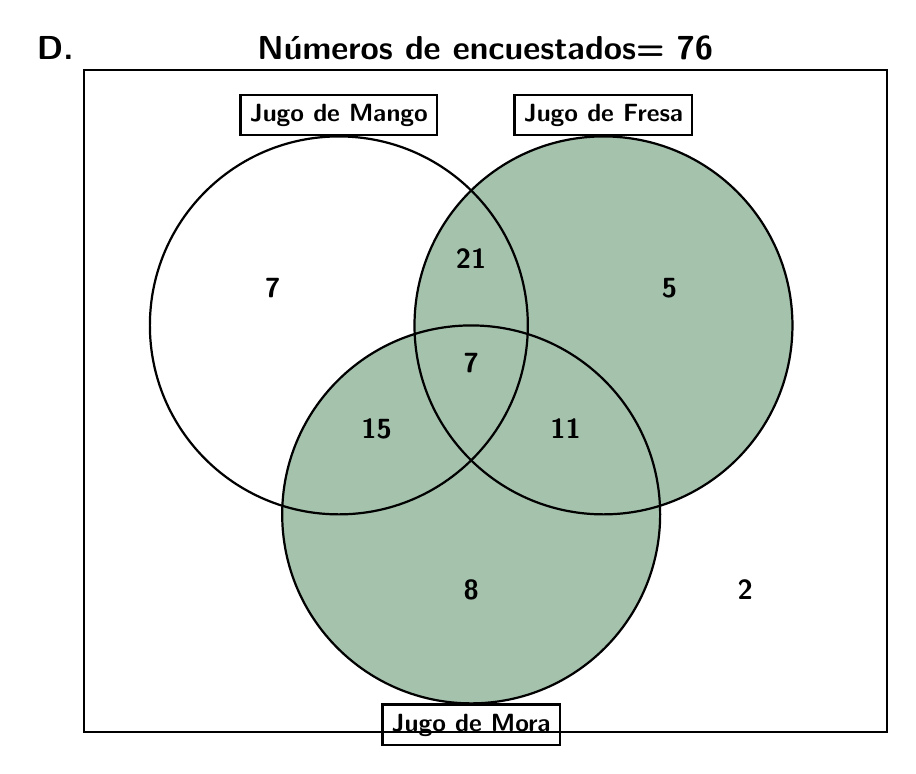
\begin{tikzpicture}[thick, scale=1.2]
		% Defines colors to match the image
		\definecolor{shadedregion}{RGB}{165, 194, 173} % A grayish green
		\definecolor{labelbox}{RGB}{255, 255, 255} % White for label boxes
		
		% Coordinates for the centers of the circles
		\coordinate (M) at (-0.8, 0.8); % Mango
		\coordinate (F) at (2.0, 0.8);  % Fresa
		\coordinate (Mo) at (0.6, -1.2); % Mora
		\def\R{2.0} % Radius of the circles
		
		% --- Shading ---
		% We need to shade the union of the Fresa and Mora sets.
		% We draw these two circles filled on the background layer.
		\begin{scope}[on background layer]
			\fill[shadedregion] (F) circle (\R);
			\fill[shadedregion] (Mo) circle (\R);
		\end{scope}
		
		% --- Circles ---
		% Draw the outlines of the circles on top of the shading
		\draw (M) circle (\R);
		\draw (F) circle (\R);
		\draw (Mo) circle (\R);
		
		% --- Labels ---
		% Labels for the sets in boxes with white background
		\node[draw, fill=labelbox, anchor=south, font=\bfseries\small] at ($(M) + (0, \R)$) {Jugo de Mango};
		\node[draw, fill=labelbox, anchor=south, font=\bfseries\small] at ($(F) + (0, \R)$) {Jugo de Fresa};
		\node[draw, fill=labelbox, anchor=north, font=\bfseries\small] at ($(Mo) - (0, \R)$) {Jugo de Mora};
		
		% --- Numbers ---
		% Place the numbers in their respective regions.
		% Positions are approximated to match the visual.
		\node[font=\bfseries] at (-1.5, 1.2) {7};  % Only Mango
		\node[font=\bfseries] at (2.7, 1.2) {5};   % Only Fresa
		\node[font=\bfseries] at (0.6, -2.0) {8};  % Only Mora
		
		\node[font=\bfseries] at (0.6, 1.5) {21};  % Mango & Fresa
		\node[font=\bfseries] at (-0.4, -0.3) {15}; % Mango & Mora
		\node[font=\bfseries] at (1.6, -0.3) {11};  % Fresa & Mora
		
		\node[font=\bfseries] at (0.6, 0.4) {7};   % All three
		
		% --- Universal Set ---
		% Draw the bounding box for the universal set
		\draw (-3.5, -3.5) rectangle (5.0, 3.5);
		
		% Number outside the sets
		\node[font=\bfseries] at (3.5, -2.0) {2};
		
		% --- Titles ---
		% Main title
		\node[anchor=south, font=\bfseries\large] at (0.75, 3.5) {Números de encuestados= 76};
		% Section letter
		\node[anchor=south east, font=\bfseries\large] at (-3.5, 3.5) {D.};
		
	\end{tikzpicture}
	
\end{document}